\documentclass{book}
\usepackage[landscape,a3paper,left=0.5cm,right=1in,top=1in,bottom=1in]{geometry}
\usepackage{amsmath}
\usepackage{xcolor}
\usepackage{tikz}
\usepackage{pgfplots}
\usepackage{booktabs}
\usepackage{multirow}
\usepackage{amsmath,amssymb}

\begin{document}

\vspace{2cm}

\begin{figure}\caption{\textsc{Equiv + Permut} for Test of 97 small instances of linear}
\vspace{0.5cm}\centering

\begin{tabular}{ccc} & gecode & coinbc\\\\\tikz{\node (a) at (0.0,2.5) {\textsc{QuadraMod}};\node (a) at (0.0,0) {};} & 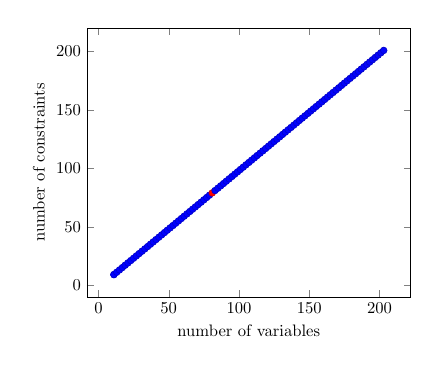
\begin{tikzpicture}[scale=0.6]
\begin{axis}[scatter, point meta=\thisrow{time}, only marks, colorbar, colorbar horizontal,colorbar style={ylabel={Time (min)}, ylabel style={rotate=270},}, colorbar to name={storedcolorbar1},, xlabel=number of variables,ylabel=number of constraints]

\addplot table[x=x,y=y]  { 
 x y time
 11 9 0.05 
 11 9 0.0 
 13 11 0.0 
 15 13 0.0 
 17 15 0.0 
 19 17 0.0 
 21 19 0.0 
 23 21 0.0 
 25 23 0.0 
 27 25 0.0 
 29 27 0.0 
 31 29 0.0 
 33 31 0.0 
 35 33 0.0 
 37 35 0.0 
 39 37 0.0 
 41 39 0.0 
 43 41 0.0 
 45 43 0.0 
 47 45 0.0 
 49 47 0.0 
 51 49 0.0 
 53 51 0.0 
 55 53 0.0 
 57 55 0.0 
 59 57 0.0 
 61 59 0.0 
 63 61 0.0 
 65 63 0.0 
 67 65 0.0 
 69 67 0.0 
 71 69 0.0 
 73 71 0.0 
 75 73 0.0 
 77 75 0.0 
 79 77 0.0 
 81 79 1440.0 
 83 81 0.0 
 85 83 0.0 
 87 85 0.0 
 89 87 0.0 
 91 89 0.0 
 93 91 0.0 
 95 93 0.0 
 97 95 0.0 
 99 97 0.0 
 101 99 0.0 
 103 101 1.0 
 105 103 1.0 
 107 105 0.0 
 109 107 1.0 
 111 109 0.0 
 113 111 0.0 
 115 113 1.0 
 117 115 1.0 
 119 117 1.0 
 121 119 1.0 
 123 121 2.0 
 125 123 1.0 
 127 125 1.0 
 129 127 1.0 
 131 129 1.0 
 133 131 2.0 
 135 133 1.0 
 137 135 1.0 
 139 137 1.0 
 141 139 2.0 
 143 141 2.0 
 145 143 4.0 
 147 145 2.0 
 149 147 3.0 
 151 149 3.0 
 153 151 3.0 
 155 153 3.0 
 157 155 3.0 
 159 157 4.0 
 161 159 3.0 
 163 161 5.0 
 165 163 4.0 
 167 165 5.0 
 169 167 8.0 
 171 169 3.0 
 173 171 3.0 
 175 173 5.0 
 177 175 6.0 
 179 177 6.0 
 181 179 5.0 
 183 181 5.0 
 185 183 6.0 
 187 185 8.0 
 189 187 6.0 
 191 189 7.0 
 193 191 7.0 
 195 193 11.0 
 197 195 9.0 
 199 197 9.0 
 201 199 11.0 
 203 201 7.0 
};

\end{axis}
\end{tikzpicture}

 & 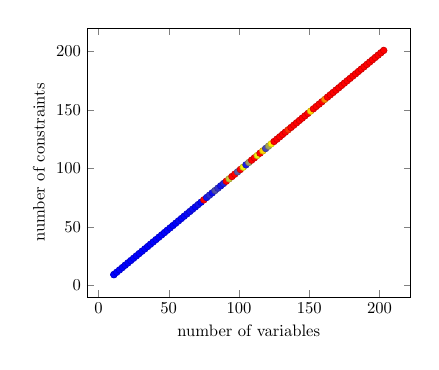
\begin{tikzpicture}[scale=0.6]
\begin{axis}[scatter, point meta=\thisrow{time}, only marks, , xlabel=number of variables,ylabel=number of constraints]

\addplot table[x=x,y=y]  { 
 x y time
 11 9 0.05 
 11 9 0.0 
 13 11 0.0 
 15 13 0.0 
 17 15 0.0 
 19 17 0.0 
 21 19 0.0 
 23 21 0.0 
 25 23 0.0 
 27 25 0.0 
 29 27 0.0 
 31 29 0.0 
 33 31 0.0 
 35 33 0.0 
 37 35 1.0 
 39 37 0.0 
 41 39 1.0 
 43 41 0.0 
 45 43 1.0 
 47 45 1.0 
 49 47 2.0 
 51 49 1.0 
 53 51 1.0 
 55 53 1.0 
 57 55 15.0 
 59 57 4.0 
 61 59 6.0 
 63 61 9.0 
 65 63 17.0 
 67 65 25.0 
 69 67 7.0 
 71 69 33.0 
 73 71 8.0 
 75 73 1440.0 
 77 75 38.0 
 79 77 75.0 
 81 79 22.0 
 83 81 150.0 
 85 83 94.0 
 87 85 36.0 
 89 87 63.0 
 91 89 1440.0 
 93 91 377.0 
 95 93 1440.0 
 97 95 1440.0 
 99 97 172.0 
 101 99 1440.0 
 103 101 461.0 
 105 103 57.0 
 107 105 295.0 
 109 107 1440.0 
 111 109 1440.0 
 113 111 446.0 
 115 113 1440.0 
 117 115 630.0 
 119 117 132.0 
 121 119 305.0 
 123 121 534.0 
 125 123 1440.0 
 127 125 1440.0 
 129 127 1440.0 
 131 129 1440.0 
 133 131 1440.0 
 135 133 1258.0 
 137 135 1440.0 
 139 137 1440.0 
 141 139 1440.0 
 143 141 1440.0 
 145 143 1440.0 
 147 145 1440.0 
 149 147 1440.0 
 151 149 633.0 
 153 151 1440.0 
 155 153 1440.0 
 157 155 1440.0 
 159 157 1440.0 
 161 159 930.0 
 163 161 1440.0 
 165 163 1440.0 
 167 165 1440.0 
 169 167 1440.0 
 171 169 1440.0 
 173 171 1440.0 
 175 173 1440.0 
 177 175 1440.0 
 179 177 1440.0 
 181 179 1440.0 
 183 181 1440.0 
 185 183 1440.0 
 187 185 1440.0 
 189 187 1440.0 
 191 189 1440.0 
 193 191 1440.0 
 195 193 1440.0 
 197 195 1440.0 
 199 197 1440.0 
 201 199 1440.0 
 203 201 1440.0 
};

\end{axis}
\end{tikzpicture}

\\
\tikz{\node (a) at (0.0,2.5) {\textsc{TheoMod}};\node (a) at (0.0,0) {};} & 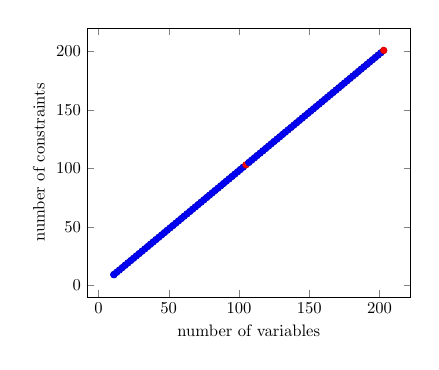
\begin{tikzpicture}[scale=0.6]
\begin{axis}[scatter, point meta=\thisrow{time}, only marks, , xlabel=number of variables,ylabel=number of constraints]

\addplot table[x=x,y=y]  { 
 x y time
 11 9 0.05 
 11 9 0.0 
 13 11 0.0 
 15 13 0.0 
 17 15 0.0 
 19 17 0.0 
 21 19 0.0 
 23 21 0.0 
 25 23 0.0 
 27 25 0.0 
 29 27 0.0 
 31 29 0.0 
 33 31 0.0 
 35 33 0.0 
 37 35 0.0 
 39 37 0.0 
 41 39 0.0 
 43 41 0.0 
 45 43 0.0 
 47 45 0.0 
 49 47 0.0 
 51 49 0.0 
 53 51 0.0 
 55 53 0.0 
 57 55 0.0 
 59 57 0.0 
 61 59 0.0 
 63 61 0.0 
 65 63 0.0 
 67 65 0.0 
 69 67 0.0 
 71 69 0.0 
 73 71 0.0 
 75 73 0.0 
 77 75 0.0 
 79 77 0.0 
 81 79 0.0 
 83 81 0.0 
 85 83 0.0 
 87 85 0.0 
 89 87 0.0 
 91 89 0.0 
 93 91 0.0 
 95 93 0.0 
 97 95 0.0 
 99 97 0.0 
 101 99 0.0 
 103 101 0.0 
 105 103 1440.0 
 107 105 0.0 
 109 107 1.0 
 111 109 1.0 
 113 111 1.0 
 115 113 1.0 
 117 115 1.0 
 119 117 1.0 
 121 119 1.0 
 123 121 1.0 
 125 123 1.0 
 127 125 1.0 
 129 127 2.0 
 131 129 2.0 
 133 131 2.0 
 135 133 3.0 
 137 135 2.0 
 139 137 3.0 
 141 139 2.0 
 143 141 3.0 
 145 143 3.0 
 147 145 3.0 
 149 147 3.0 
 151 149 4.0 
 153 151 5.0 
 155 153 4.0 
 157 155 5.0 
 159 157 4.0 
 161 159 5.0 
 163 161 5.0 
 165 163 6.0 
 167 165 6.0 
 169 167 7.0 
 171 169 7.0 
 173 171 8.0 
 175 173 6.0 
 177 175 7.0 
 179 177 10.0 
 181 179 9.0 
 183 181 11.0 
 185 183 10.0 
 187 185 10.0 
 189 187 11.0 
 191 189 12.0 
 193 191 13.0 
 195 193 12.0 
 197 195 12.0 
 199 197 13.0 
 201 199 15.0 
 203 201 1440.0 
};

\end{axis}
\end{tikzpicture}

 & 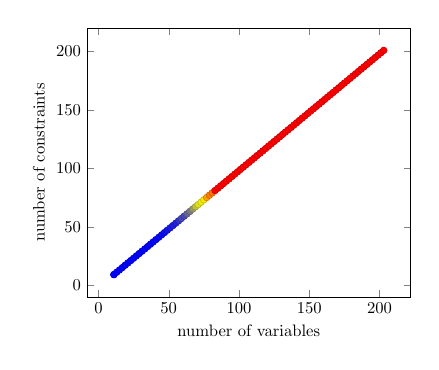
\begin{tikzpicture}[scale=0.6]
\begin{axis}[scatter, point meta=\thisrow{time}, only marks, , xlabel=number of variables,ylabel=number of constraints]

\addplot table[x=x,y=y]  { 
 x y time
 11 9 0.05 
 11 9 0.0 
 13 11 0.0 
 15 13 0.0 
 17 15 0.0 
 19 17 0.0 
 21 19 0.0 
 23 21 0.0 
 25 23 0.0 
 27 25 1.0 
 29 27 1.0 
 31 29 1.0 
 33 31 3.0 
 35 33 3.0 
 37 35 6.0 
 39 37 10.0 
 41 39 10.0 
 43 41 15.0 
 45 43 18.0 
 47 45 24.0 
 49 47 35.0 
 51 49 46.0 
 53 51 57.0 
 55 53 60.0 
 57 55 90.0 
 59 57 132.0 
 61 59 133.0 
 63 61 187.0 
 65 63 226.0 
 67 65 281.0 
 69 67 361.0 
 71 69 422.0 
 73 71 445.0 
 75 73 564.0 
 77 75 828.0 
 79 77 965.0 
 81 79 999.0 
 83 81 1440.0 
 85 83 1440.0 
 87 85 1440.0 
 89 87 1440.0 
 91 89 1440.0 
 93 91 1440.0 
 95 93 1440.0 
 97 95 1440.0 
 99 97 1440.0 
 101 99 1440.0 
 103 101 1440.0 
 105 103 1440.0 
 107 105 1440.0 
 109 107 1440.0 
 111 109 1440.0 
 113 111 1440.0 
 115 113 1440.0 
 117 115 1440.0 
 119 117 1440.0 
 121 119 1440.0 
 123 121 1440.0 
 125 123 1440.0 
 127 125 1440.0 
 129 127 1440.0 
 131 129 1440.0 
 133 131 1440.0 
 135 133 1440.0 
 137 135 1440.0 
 139 137 1440.0 
 141 139 1440.0 
 143 141 1440.0 
 145 143 1440.0 
 147 145 1440.0 
 149 147 1440.0 
 151 149 1440.0 
 153 151 1440.0 
 155 153 1440.0 
 157 155 1440.0 
 159 157 1440.0 
 161 159 1440.0 
 163 161 1440.0 
 165 163 1440.0 
 167 165 1440.0 
 169 167 1440.0 
 171 169 1440.0 
 173 171 1440.0 
 175 173 1440.0 
 177 175 1440.0 
 179 177 1440.0 
 181 179 1440.0 
 183 181 1440.0 
 185 183 1440.0 
 187 185 1440.0 
 189 187 1440.0 
 191 189 1440.0 
 193 191 1440.0 
 195 193 1440.0 
 197 195 1440.0 
 199 197 1440.0 
 201 199 1440.0 
 203 201 1440.0 
};

\end{axis}
\end{tikzpicture}

\\
\\\\
\multicolumn{3}{c}{\ref{storedcolorbar1}}\end{tabular}\end{figure}

\newpage

\begin{figure}\caption{\textsc{Non-Equiv + Permut} for Test of 97 small instances of linear}
\vspace{0.5cm}\centering

\begin{tabular}{ccc} & gecode & coinbc\\\\\tikz{\node (a) at (0.0,2.5) {\textsc{QuadraMod}};\node (a) at (0.0,0) {};} & 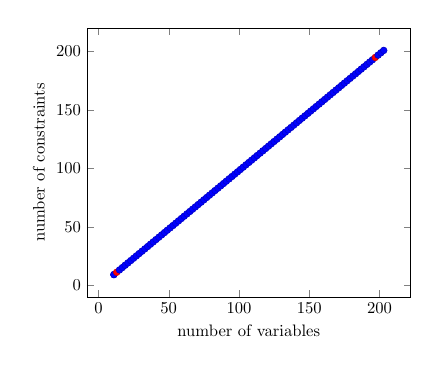
\begin{tikzpicture}[scale=0.6]
\begin{axis}[scatter, point meta=\thisrow{time}, only marks, colorbar, colorbar horizontal,colorbar style={ylabel={Time (min)}, ylabel style={rotate=270},}, colorbar to name={storedcolorbar2},, xlabel=number of variables,ylabel=number of constraints]

\addplot table[x=x,y=y]  { 
 x y time
 11 9 0.05 
 11 9 0.0 
 13 11 1440.0 
 15 13 0.0 
 17 15 0.0 
 19 17 0.0 
 21 19 0.0 
 23 21 0.0 
 25 23 0.0 
 27 25 0.0 
 29 27 0.0 
 31 29 0.0 
 33 31 0.0 
 35 33 0.0 
 37 35 0.0 
 39 37 0.0 
 41 39 0.0 
 43 41 0.0 
 45 43 0.0 
 47 45 0.0 
 49 47 0.0 
 51 49 0.0 
 53 51 0.0 
 55 53 0.0 
 57 55 0.0 
 59 57 0.0 
 61 59 0.0 
 63 61 0.0 
 65 63 0.0 
 67 65 0.0 
 69 67 0.0 
 71 69 0.0 
 73 71 0.0 
 75 73 0.0 
 77 75 0.0 
 79 77 0.0 
 81 79 0.0 
 83 81 0.0 
 85 83 0.0 
 87 85 0.0 
 89 87 0.0 
 91 89 0.0 
 93 91 0.0 
 95 93 0.0 
 97 95 0.0 
 99 97 0.0 
 101 99 0.0 
 103 101 0.0 
 105 103 0.0 
 107 105 0.0 
 109 107 1.0 
 111 109 1.0 
 113 111 0.0 
 115 113 1.0 
 117 115 1.0 
 119 117 1.0 
 121 119 2.0 
 123 121 1.0 
 125 123 1.0 
 127 125 1.0 
 129 127 1.0 
 131 129 1.0 
 133 131 1.0 
 135 133 1.0 
 137 135 2.0 
 139 137 2.0 
 141 139 1.0 
 143 141 3.0 
 145 143 4.0 
 147 145 1.0 
 149 147 1.0 
 151 149 2.0 
 153 151 2.0 
 155 153 2.0 
 157 155 5.0 
 159 157 2.0 
 161 159 3.0 
 163 161 3.0 
 165 163 2.0 
 167 165 3.0 
 169 167 3.0 
 171 169 2.0 
 173 171 3.0 
 175 173 3.0 
 177 175 4.0 
 179 177 4.0 
 181 179 4.0 
 183 181 5.0 
 185 183 3.0 
 187 185 3.0 
 189 187 4.0 
 191 189 4.0 
 193 191 10.0 
 195 193 5.0 
 197 195 1440.0 
 199 197 5.0 
 201 199 7.0 
 203 201 6.0 
};

\end{axis}
\end{tikzpicture}

 & 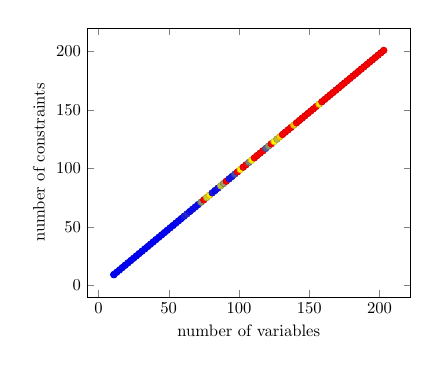
\begin{tikzpicture}[scale=0.6]
\begin{axis}[scatter, point meta=\thisrow{time}, only marks, , xlabel=number of variables,ylabel=number of constraints]

\addplot table[x=x,y=y]  { 
 x y time
 11 9 0.05 
 11 9 0.0 
 13 11 0.0 
 15 13 0.0 
 17 15 0.0 
 19 17 0.0 
 21 19 0.0 
 23 21 0.0 
 25 23 0.0 
 27 25 0.0 
 29 27 0.0 
 31 29 0.0 
 33 31 0.0 
 35 33 0.0 
 37 35 8.0 
 39 37 0.0 
 41 39 1.0 
 43 41 1.0 
 45 43 0.0 
 47 45 12.0 
 49 47 1.0 
 51 49 8.0 
 53 51 1.0 
 55 53 1.0 
 57 55 15.0 
 59 57 3.0 
 61 59 50.0 
 63 61 72.0 
 65 63 19.0 
 67 65 21.0 
 69 67 26.0 
 71 69 18.0 
 73 71 254.0 
 75 73 1440.0 
 77 75 383.0 
 79 77 561.0 
 81 79 43.0 
 83 81 21.0 
 85 83 32.0 
 87 85 365.0 
 89 87 294.0 
 91 89 1440.0 
 93 91 41.0 
 95 93 38.0 
 97 95 140.0 
 99 97 1440.0 
 101 99 519.0 
 103 101 1440.0 
 105 103 1440.0 
 107 105 240.0 
 109 107 552.0 
 111 109 1440.0 
 113 111 1440.0 
 115 113 1440.0 
 117 115 1440.0 
 119 117 170.0 
 121 119 278.0 
 123 121 1440.0 
 125 123 508.0 
 127 125 356.0 
 129 127 652.0 
 131 129 1440.0 
 133 131 1440.0 
 135 133 1440.0 
 137 135 1440.0 
 139 137 716.0 
 141 139 1440.0 
 143 141 1440.0 
 145 143 1440.0 
 147 145 1440.0 
 149 147 1440.0 
 151 149 1440.0 
 153 151 1440.0 
 155 153 1440.0 
 157 155 602.0 
 159 157 1440.0 
 161 159 1440.0 
 163 161 1440.0 
 165 163 1440.0 
 167 165 1440.0 
 169 167 1440.0 
 171 169 1440.0 
 173 171 1440.0 
 175 173 1440.0 
 177 175 1440.0 
 179 177 1440.0 
 181 179 1440.0 
 183 181 1440.0 
 185 183 1440.0 
 187 185 1440.0 
 189 187 1440.0 
 191 189 1440.0 
 193 191 1440.0 
 195 193 1440.0 
 197 195 1440.0 
 199 197 1440.0 
 201 199 1440.0 
 203 201 1440.0 
};

\end{axis}
\end{tikzpicture}

\\
\tikz{\node (a) at (0.0,2.5) {\textsc{TheoMod}};\node (a) at (0.0,0) {};} & 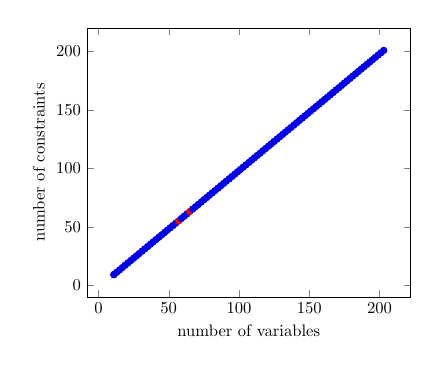
\begin{tikzpicture}[scale=0.6]
\begin{axis}[scatter, point meta=\thisrow{time}, only marks, , xlabel=number of variables,ylabel=number of constraints]

\addplot table[x=x,y=y]  { 
 x y time
 11 9 0.05 
 11 9 0.0 
 13 11 0.0 
 15 13 0.0 
 17 15 0.0 
 19 17 0.0 
 21 19 0.0 
 23 21 0.0 
 25 23 0.0 
 27 25 0.0 
 29 27 0.0 
 31 29 0.0 
 33 31 0.0 
 35 33 0.0 
 37 35 0.0 
 39 37 0.0 
 41 39 0.0 
 43 41 0.0 
 45 43 0.0 
 47 45 0.0 
 49 47 0.0 
 51 49 0.0 
 53 51 0.0 
 55 53 0.0 
 57 55 1440.0 
 59 57 0.0 
 61 59 0.0 
 63 61 0.0 
 65 63 1440.0 
 67 65 0.0 
 69 67 0.0 
 71 69 0.0 
 73 71 0.0 
 75 73 0.0 
 77 75 0.0 
 79 77 0.0 
 81 79 0.0 
 83 81 0.0 
 85 83 0.0 
 87 85 0.0 
 89 87 0.0 
 91 89 0.0 
 93 91 0.0 
 95 93 0.0 
 97 95 0.0 
 99 97 0.0 
 101 99 0.0 
 103 101 0.0 
 105 103 0.0 
 107 105 0.0 
 109 107 0.0 
 111 109 0.0 
 113 111 0.0 
 115 113 0.0 
 117 115 0.0 
 119 117 0.0 
 121 119 0.0 
 123 121 0.0 
 125 123 0.0 
 127 125 0.0 
 129 127 0.0 
 131 129 0.0 
 133 131 0.0 
 135 133 0.0 
 137 135 0.0 
 139 137 0.0 
 141 139 0.0 
 143 141 0.0 
 145 143 0.0 
 147 145 0.0 
 149 147 0.0 
 151 149 0.0 
 153 151 0.0 
 155 153 0.0 
 157 155 0.0 
 159 157 0.0 
 161 159 0.0 
 163 161 0.0 
 165 163 0.0 
 167 165 0.0 
 169 167 0.0 
 171 169 0.0 
 173 171 0.0 
 175 173 0.0 
 177 175 0.0 
 179 177 0.0 
 181 179 0.0 
 183 181 0.0 
 185 183 0.0 
 187 185 0.0 
 189 187 0.0 
 191 189 0.0 
 193 191 0.0 
 195 193 0.0 
 197 195 0.0 
 199 197 0.0 
 201 199 0.0 
 203 201 0.0 
};

\end{axis}
\end{tikzpicture}

 & 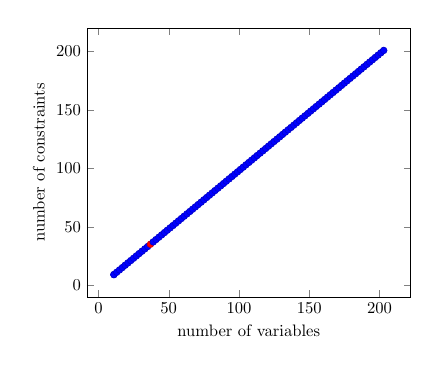
\begin{tikzpicture}[scale=0.6]
\begin{axis}[scatter, point meta=\thisrow{time}, only marks, , xlabel=number of variables,ylabel=number of constraints]

\addplot table[x=x,y=y]  { 
 x y time
 11 9 0.05 
 11 9 0.0 
 13 11 0.0 
 15 13 0.0 
 17 15 0.0 
 19 17 0.0 
 21 19 0.0 
 23 21 0.0 
 25 23 0.0 
 27 25 0.0 
 29 27 0.0 
 31 29 0.0 
 33 31 0.0 
 35 33 0.0 
 37 35 5.0 
 39 37 0.0 
 41 39 0.0 
 43 41 0.0 
 45 43 0.0 
 47 45 0.0 
 49 47 0.0 
 51 49 0.0 
 53 51 0.0 
 55 53 0.0 
 57 55 0.0 
 59 57 0.0 
 61 59 0.0 
 63 61 0.0 
 65 63 0.0 
 67 65 0.0 
 69 67 0.0 
 71 69 0.0 
 73 71 0.0 
 75 73 0.0 
 77 75 0.0 
 79 77 0.0 
 81 79 0.0 
 83 81 0.0 
 85 83 0.0 
 87 85 0.0 
 89 87 0.0 
 91 89 0.0 
 93 91 0.0 
 95 93 0.0 
 97 95 0.0 
 99 97 0.0 
 101 99 0.0 
 103 101 0.0 
 105 103 0.0 
 107 105 0.0 
 109 107 0.0 
 111 109 0.0 
 113 111 0.0 
 115 113 0.0 
 117 115 0.0 
 119 117 0.0 
 121 119 0.0 
 123 121 0.0 
 125 123 0.0 
 127 125 0.0 
 129 127 0.0 
 131 129 0.0 
 133 131 0.0 
 135 133 0.0 
 137 135 0.0 
 139 137 0.0 
 141 139 0.0 
 143 141 0.0 
 145 143 0.0 
 147 145 0.0 
 149 147 0.0 
 151 149 0.0 
 153 151 0.0 
 155 153 0.0 
 157 155 0.0 
 159 157 0.0 
 161 159 0.0 
 163 161 0.0 
 165 163 0.0 
 167 165 0.0 
 169 167 0.0 
 171 169 0.0 
 173 171 0.0 
 175 173 0.0 
 177 175 0.0 
 179 177 0.0 
 181 179 0.0 
 183 181 0.0 
 185 183 0.0 
 187 185 0.0 
 189 187 0.0 
 191 189 0.0 
 193 191 0.0 
 195 193 0.0 
 197 195 0.0 
 199 197 0.0 
 201 199 0.0 
 203 201 0.0 
};

\end{axis}
\end{tikzpicture}

\\
\\\\
\multicolumn{3}{c}{\ref{storedcolorbar2}}\end{tabular}\end{figure}

\newpage

\end{document}